\section{Typed Decision Models}
\label{sec:models}

\subsection{The Interface}
\label{sec:jev}

To see how these decisions are expressed in practice, we use Jev~1.13 as a concrete example, following TypeSafe's public documentation~\cite{typesafe2026docs}.

\noindent\textbf{Calls and question types.} A call carries a \emph{state}, which is text, a JSON object or an array of text values. It also carries a set of keyed questions of three types: 1) a \texttt{choice} question selects one option from a caller-defined set of at most 255 options, and the answer gives a probability for every option; 2) a \texttt{score} question places the state on an ordered rubric of 2 to 10 levels, and the answer gives a probability for every level and the probability-weighted level; and 3) a Boolean question, which TypeSafe calls \texttt{noul}, asks whether a statement is true, and the answer is the probability of yes. Types can be mixed in one call. The questions of a call are evaluated against the state independently of one another.

\noindent\textbf{Pricing and versions.} The service is priced per input token, and output tokens are free. The same weights serve every account, so a caller adapts Jev only through the state and the text of its questions. Model aliases resolve to versioned identifiers, and the documentation advises pinning a version whenever thresholds have been tuned. Because the service is hosted, every state is sent to TypeSafe. When the state must stay on the team's own infrastructure, only the open-weight rows of Table~\ref{tab:implementations} apply.

\noindent\textbf{Training.} TypeSafe has published no technical report, weights, parameter count, architecture or description of its training data. Its documentation states that customer requests are not used for training. The one named training method is reinforcement learning for calibrated decisions (RLCD). TypeSafe describes RLCD as training the model to return decisions and calibrated probabilities instead of generated text.

\noindent\textbf{Documented limitations.} Jev reads instructions literally and is unreliable on counting, arithmetic, date comparisons and questions that need several hops of reasoning. Its accuracy falls when the state contains unrelated material. It does not treat the state as hostile, so text in the state can steer its answer. A Boolean question and its negation need not receive complementary probabilities. TypeSafe lists these limitations for \texttt{jev-1.13} and pairs each with a workaround, such as keeping arithmetic in code.

\noindent\textbf{A worked call.} Fig.~\ref{fig:interface} shows one call with illustrative values. The state is an agent's proposed tool call together with the user's request. The caller asks one question of each type, and the model returns one distribution per question. The caller's code then applies a threshold to each answer and combines the results. The thresholds, and the decision to act, abstain or escalate, belong to the caller rather than to the model.

\begin{figure*}[t]
\centering
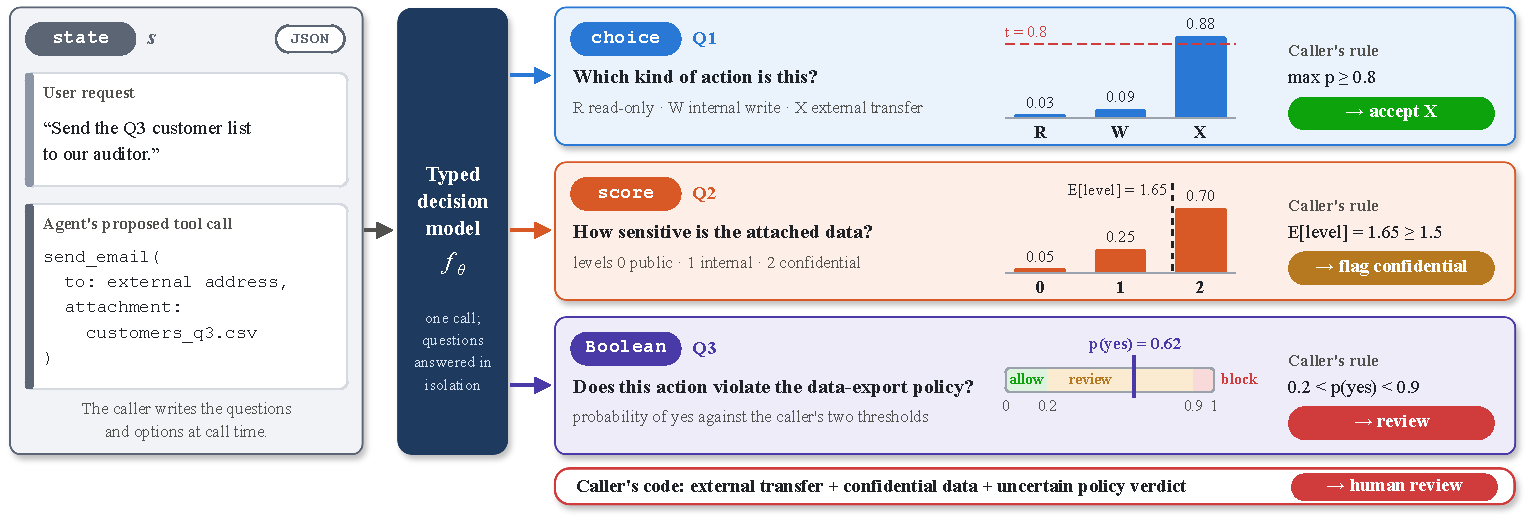
\includegraphics[width=\textwidth]{figures/fig_interface.pdf}
\caption{A worked call to a typed decision model, with illustrative rather than measured values. One state is evaluated against three questions, one of each type. The model returns a distribution over each question's closed answer set: bars show the \texttt{choice} and \texttt{score} distributions, and the Boolean answer is the probability of yes, shown against the caller's allow and block thresholds (shaded band: review). The caller, not the model, sets the thresholds and the rule that combines them.}
\label{fig:interface}
\end{figure*}

\subsection{Properties for Evaluating Typed Decisions}
\label{sec:contract}

We judge a typed decision model by four properties: type safety (P1), calibration (P2), invariance (P3) and cost (P4).

\noindent\textbf{Type safety (P1).} Every answer lies in the declared answer set. This is structural validity, not correctness.

\noindent\textbf{Calibration (P2).} For a \texttt{choice} question, predictions assigned a given top probability should be correct at that rate. The same condition applies to the probability of yes for Boolean questions and to each cumulative event for \texttt{score} questions. Calibration is measured on a deployment distribution, so a model calibrated for one question and one traffic mix need not be calibrated for another, or within every subgroup. The studies in Section~\ref{sec:evidence} report the expected calibration error (ECE), a binned estimate of this gap.

\noindent\textbf{Invariance (P3).} Reordering the options should not change the probability each option receives. Renaming the options while their definitions are held fixed should not change it either. P3 also covers coherence: a question and its negation should receive complementary probabilities.

\noindent\textbf{Cost (P4).} Cost covers forward passes, network round trips, latency and price per decision. Reports should state what the latency includes, for example model time only or the full round trip.

Type safety is an interface requirement. Calibration, invariance and cost describe behavior that must be measured rather than assumed. Constrained decoding also guarantees type safety~\cite{willard2023efficient}, but the model still generates tokens and exposes probabilities only where the provider returns token log-probabilities. LLM judges accept a rubric at call time~\cite{kim2024prometheus2,liu2023geval}, but they usually report a score or verdict, often with a rationale, rather than a calibrated probability~\cite{gu2024survey}.

Software acts on a decision through an \emph{acceptance rule} that the caller sets. A \texttt{choice} is typically executed when its top probability exceeds a threshold and escalated otherwise. A Boolean gate that asks whether an action is unsafe can use two thresholds. It allows the action below the lower one, blocks it above the upper one, and asks for human review in between. When low-confidence decisions are deferred in this way, the model acts as a selective predictor~\cite{geifman2017selective}. We call the share of decisions resolved without human review or escalation the \emph{automation coverage}. For a Boolean gate, it includes both automatic allows and automatic blocks.

\subsection{Implementations}
\label{sec:implementations}
\begin{table}[!t]
\centering
\caption{Implementations of the typed decision interface, grouped by mechanism family. ``User labels'' counts the labeled examples a user supplies per new question to obtain probabilities; developer training data are excluded. Every row still needs labeled evidence to set an acceptance rule for a risk target (Section~\ref{sec:adaptation}). ``Passes'' counts model passes for one question. L0, L1 and L2 are AnyJev's zero-label, temperature-fitted and closed-form-head levels, with label counts as stated by its developers. $K$: number of options.}
\label{tab:implementations}
\footnotesize
\setlength{\tabcolsep}{3pt}
\renewcommand{\arraystretch}{1.05}
\begin{tabularx}{\columnwidth}{@{}>{\raggedright\arraybackslash\hspace{0pt}}p{1.35cm}>{\raggedright\arraybackslash\hspace{0pt}}X>{\raggedright\arraybackslash\hspace{0pt}}p{1.3cm}>{\raggedright\arraybackslash\hspace{0pt}}p{1.75cm}@{}}
\toprule
\tblhead \thd{System} & \thd{Mechanism and training} & \thd{User labels} & \thd{Passes} \\
\midrule
\tblgroup{4}{Hosted, closed weights}
Jev 1.13~\cite{typesafe2026docs} & Vendor-trained with RLCD; unpublished & 0 & One API call, which several questions can share \\
\midrule
\tblgroup{4}{Open weights: trained encoder heads}
Laya~\cite{convai2026laya} & Fine-tuned ModernBERT or mmBERT & 0; developers advise task fine-tuning and local temperature fitting & One encoder forward pass \\
\midrule
\tblgroup{4}{Open weights: fine-tuned decoders}
Kev~\cite{palmer2026kev} & Pointer head on Qwen3.5 or Qwen3.8; LoRA, full fine-tuning at 27B & 0 & One prefill \\
Nimble~\cite{bespoke2026nimble} & LoRA on Qwen3.5-9B & 0 & One prefill \\
Decider~\cite{mapika2026decider} & Fine-tuned Qwen3.5; also a Gemma-4 LoRA and stock-model readout variants & 0 & One prefill \\
\midrule
\tblgroup{4}{Open weights: readout from frozen models}
SemIf~\cite{lee2026semif} & Logit readout from frozen checkpoints & 0 & One prefill \\
AnyJev~\cite{nokia2026anyjev} & Debiased readout (L0); temperature (L1); closed-form head, no gradient training (L2) & 0 (L0); 100--500 (L1); 100--300 (L2) & Up to $K$ prompts sharing the state prefix (L0, L1); one partial forward pass (L2) \\
\bottomrule
\end{tabularx}
\end{table}


Beyond Jev, open implementations fall into three families (Table~\ref{tab:implementations}): 1) trained encoder heads, such as Laya, which fine-tunes ModernBERT-class encoders~\cite{convai2026laya,warner2024smarter}; 2) fine-tuned decoders, such as Kev, Nimble and trained Decider variants, which adapt open decoder models~\cite{palmer2026kev,bespoke2026nimble,mapika2026decider}; and 3) readout from frozen open models, such as SemIf, AnyJev and stock-weight Decider variants~\cite{lee2026semif,nokia2026anyjev,mapika2026decider}. Laya, Kev, Nimble and Decider expose endpoints modeled on TypeSafe's request format~\cite{convai2026laya,palmer2026kev,bespoke2026nimble,mapika2026decider}, although supported inputs and confidence fields differ. Compatibility does not establish equivalent decision behavior. Most calibration claims for the open implementations also come from their own developers.
